\begin{appendices}

%Some Table of Contents entry formatting
\addtocontents{toc}{\protect\renewcommand{\protect\cftchappresnum}{\appendixname\space}}
\addtocontents{toc}{\protect\renewcommand{\protect\cftchapnumwidth}{6em}}

%Begin individual appendices, separated as chapters

% \begin{itemize}
% 	\item Include operational details or a manual of your prototype as an appendix. Most of your prototypes will be disassembled for parts, so this manual should include sufficient details to recreate prototype
% 	\item Include all drawings: Circuit schematics, PCB layouts, CAD designs
% 	\item Include code (if necessary), software scripts or hardware drivers, etc.
% 	\item HW component details , include all details like data sheet, vendor name \& cost.
% 	\item Any other data related to your project which can be useful for future use.
% \end{itemize}

\chapter{Timeline with Milestones}
\label{sec:timeline}

This project is scheduled over the duration of a full academic year, from August to May. This is detailed in the Gantt chart (Figure~\ref{fig:gantt_chart}), with May kept as buffer. This way, the risks inherent to the project can be minimized, particularly by prioritizing the prototype before final fabrication.

% --- Figure 4.1: Gantt Chart ---
\begin{figure}[H]
  \centering
  % --- ACTION: Take a screenshot of Slide 45 from your *first* pitch deck ---
  % --- Save it as "gantt_chart.png" in your project folder ---
  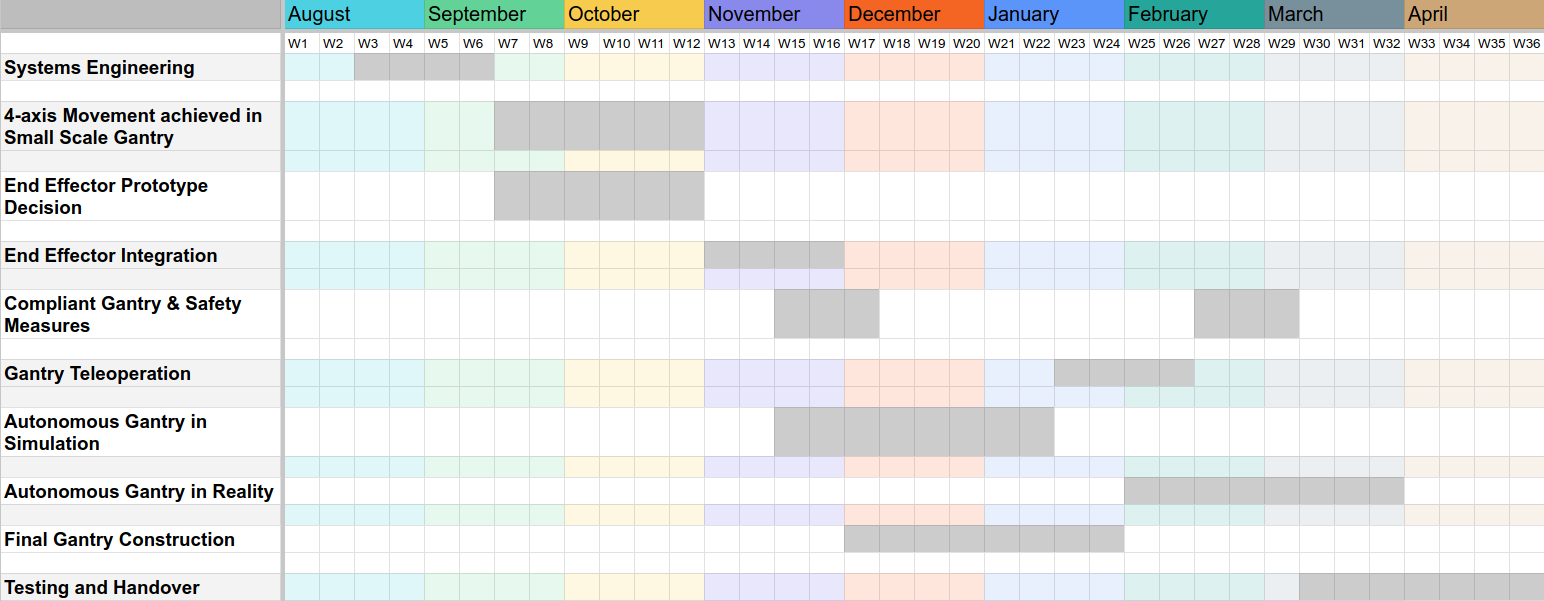
\includegraphics[width=\textwidth]{figures/gantt_chart.png}
  
  % \framebox{\parbox{0.8\textwidth}{\centering
  %   \vspace{8cm}
  %   \textbf{Figure 4.1 Placeholder} \\
  %   \small\textit{Project Timeline / Gantt Chart (from Pitch Deck, Slide 45).}
  %   \vspace{8cm}
  % }}
  \caption{Project management timeline.}
  \label{fig:gantt_chart}
\end{figure}

\chapter{Estimated Budget and Bill of Materials}
\label{sec:budget}

The total estimated budget for the project is \textbf{Rs 1,779,400}, which is within the \textbf{Rs 1.8M} financial constraint. This budget is based on the detailed Bill of Materials (BOM) shown in Table~\ref{tab:bom}, which was sourced from the team's initial budget analysis. This is approved from Dawlance.

Note that some of the items differ from the final design, due to changes in the design. However, the final design adheres to the  total budget.

% --- Table 4.2: Bill of Materials ---
\renewcommand{\arraystretch}{0.9} % Sets row height to 1.5x text height
\begin{table}[H]
  \centering
  \caption{Estimated Bill of Materials (BOM) and Budget}
  \label{tab:bom}
  \begin{tabular}{@{}l l r r r@{}}
    \toprule
    \textbf{Subsystem} & \textbf{Item} & \textbf{Qty} & \textbf{Unit (Rs)} & \textbf{Total (Rs)} \\
    \midrule
    \textbf{Materials} & Aluminium 6061 pipes/kg & 300 & 797 & 239,127 \\
     & Ball Screw & 4 & 55,512 & 222,047 \\
     & Blank Rods/kg & 10 & 854 & 8,540 \\
    \addlinespace
    \textbf{Computer} & Jetson Orin Nano & 1 & 79,709 & 79,709 \\
     & Realsense Depth Camera & 2 & 89,388 & 178,776 \\
    \addlinespace
    \textbf{Vacuum System} & Vacuum pump & 1 & 35,584 & 35,584 \\
     & Vacuum control & 1 & 7,971 & 7,971 \\
     & Suction cups & 10 & 1,423 & 14,234 \\
     & Vacuum tubing & 5 & 996 & 4,982 \\
    \addlinespace
    \textbf{End Effector} & STM32H7 & 1 & 15,372 & 15,372 \\
     & Encoder + Motor & 12 & 14,518 & 174,221 \\
     & Worm Gears & 8 & 1,082 & 8,654 \\
     & Timing belts & 4 & 3,416 & 13,664 \\
     & Pulleys & 10 & 1,708 & 17,081 \\
     & Bearings & 20 & 421 & 8,426 \\
     & Pressure sensors & 4 & 854 & 3,416 \\
    \addlinespace
    \textbf{Gantry Control} & Torque control driver & 1 & 142,338 & 142,338 \\
     & Encoder + Motors & 4 & 22,489 & 89,957 \\
     & Linear Encoders & 4 & 11,387 & 45,548 \\
     & 3-axis Force sensor & 1 & 113,870 & 113,870 \\
    \midrule
    \textbf{Subtotal} & & & & \textbf{Rs 1,423,520} \\
    \textbf{Contingency (25\%)} & & & & \textbf{Rs 355,880} \\
    \midrule
    \textbf{Total Estimated Budget} & & & & \textbf{Rs 1,779,400} \\
    \bottomrule
  \end{tabular}
\end{table}



\end{appendices}

